\chapter{Magnetics}\label{ch:magnetics}

\epigraph{ ``More than the diamond Koh-i-noor, which glitters among their crown jewels, they prize the dull pebble which is wiser than a man, whose poles turn themselves to the poles of the world, and whose axis is parallel to the axis of the world.  Now, their toys are steam and galvanism.''}
{{\normalfont ---\ Ralph Waldo Emerson}, English Traits}

\section{Introduction}
Magnetics is often introduced as a close relative of gravity, and mathematically the two methods share much in common: both are potential-field techniques governed by the same class of equations and both rely on superposition to relate subsurface sources to surface observations. The similarity ends, however, at the nature of the source. Whereas gravity responds to a scalar property (density), magnetic anomalies arise from vector magnetization, making magnetics fundamentally more complex and, in many cases, less intuitive than gravity.

Magnetic fields measured in geophysical surveys reflect the distribution of magnetized material within the Earth, but magnetization itself depends on multiple factors: the strength and direction of the Earth's magnetic field, the magnetic susceptibility of rocks, and the presence or absence of remanent magnetization. In contrast to density, magnetic properties are controlled by trace abundances of Fe-Ti oxide minerals, which are unevenly distributed in the crust and may be entirely absent in some lithologies. As a result, magnetic sources can be spatially discontinuous, strongly lithology-dependent, and highly sensitive to thermal and alteration history.

Because magnetization is directional, magnetic anomalies are not necessarily centered over their sources and can change sign depending on latitude, source orientation, and magnetization direction. Geometry alone is therefore insufficient to interpret magnetic data: direction matters. This directional dependence introduces additional ambiguity beyond that encountered in gravity, where source geometry dominates interpretation. Understanding how vector sources interact with geometry and observation geometry is central to magnetic interpretation.

In many exploration-scale applications, magnetics is treated under the assumption of induced magnetization aligned with the present-day Earth's field, allowing the magnetic field to be modeled as a steady-state potential field. This approximation enables the use of canonical source models, spectral transformations, and forward modeling approaches analogous to those used in gravity. However, it is an approximation rather than a universal truth, and its limitations must be kept in mind throughout interpretation.

In this chapter, magnetics is developed as a potential-field method whose complexity arises not from the governing equations, but from the physics of its sources. We emphasize the role of magnetic material properties, the consequences of vector superposition, and the geological meaning of common magnetic transformations. Magnetics provides a natural bridge between gravity and more advanced topics such as Fourier methods and inversion, while also motivating extension topics---such as paleomagnetism (Ch.~\ref{ch:paleomag})---that address fundamentally different geological questions using magnetic principles.

\ntextbox{Key Concepts}{
\begin{itemize}
    \item \textbf{Magnetics is a potential-field method, but its sources are vectorial rather than scalar.}

    Magnetic anomalies arise from magnetization vectors whose magnitude and direction matter, making magnetics fundamentally more complex and less intuitive than gravity.

    \textit{How does the vector nature of magnetization change interpretation compared to scalar density contrasts?}

    \item \textbf{Magnetic anomalies result from superposition of magnetization vectors.}

    Observed fields represent the sum of contributions from all magnetized bodies, but vector superposition means amplitudes and polarities depend on direction as well as geometry.

    \textit{How can vector superposition cause magnetic anomalies to reinforce, cancel, or shift spatially?}

    \item \textbf{Magnetic properties are controlled by trace mineralogy and are unevenly distributed in the crust.}

    Susceptibility and magnetization depend primarily on Fe--Ti oxide minerals, which may be concentrated, altered, or absent depending on lithology and history.

    \textit{Why does this make magnetic data less continuous and more lithology-dependent than gravity data?}

    \item \textbf{Geometry alone is insufficient for magnetic interpretation; direction matters.}

    Magnetic anomalies may be displaced from their sources and can change sign depending on latitude, magnetization direction, and observation geometry.

    \textit{Why can two geometrically identical bodies produce very different magnetic signatures?}

    \item \textbf{Most exploration-scale magnetic modeling assumes induced magnetization aligned with the Earth's field.}

    This approximation allows magnetics to be treated as a steady-state potential field, but it is not universally valid and can break down in the presence of strong remanence.

    \textit{Under what geological conditions is the induced-field assumption most likely to fail?}

    \item \textbf{Thermal structure limits magnetic sources through Curie temperature effects.}

    Magnetization is lost above the Curie temperature, imposing a thermal cutoff depth that links magnetics directly to geothermics and lithospheric structure.

    \textit{How does thermal structure influence the depth extent of magnetic sources?}

    \item \textbf{Canonical magnetic source models are abstractions that build intuition and constrain interpretation.}

    Dipoles, prisms, and related models are not realistic representations of geology, but they clarify scaling behavior, directional effects, and bounding limits on plausible source geometries.

    \textit{How can simplified magnetic models place limits on source depth and orientation?}

    \item \textbf{Magnetic transformations are most naturally understood in the spectral domain.}

    Operations such as reduction to the pole, continuation, and filtering are conceptually spectral, even when applied in the space domain.

    \textit{Why does Fourier-domain thinking simplify many magnetic operations?}

    \item \textbf{Magnetic interpretation is strongly non-unique and often more ambiguous than gravity.}

    Directional effects, remanence, and material heterogeneity introduce additional trade-offs that cannot be resolved from magnetic data alone.

    \textit{What complementary data or assumptions are needed to reduce magnetic ambiguity?}

    \item \textbf{Magnetics provides a bridge to Fourier methods, inversion, and paleomagnetism.}

    The complexity of magnetic sources motivates spectral techniques and formal inversion, while also leading naturally to extension topics that address geological history rather than structure alone.

    \textit{How does magnetics connect potential-field methods to broader Earth science questions?}
\end{itemize}
}{core}

\section{Mathematical symbols and units}

\begin{table}[hbt]
    \caption{Definitions of symbols.\vspace{2pt}}
    \label{tab:gravsym}
    \begin{tabular*}{\textwidth}{@{\extracolsep{\fill}}cll}
        \toprule
        Symbol &
        Quantity &
        SI Unit \\
        \midrule
        $x$, $y$, $z$   & distance                          & meter, \si{m} \\
        $r$             & radius                            & meter, \si{m} \\
        $q$             & magnetic pole strength            & \si{A.m} \\
        $\vb{m}$      & magnetic dipole moment            & \si{A.m^{2}} \\
        $\vb{M}$      & magnetization                     & \si{A.m^{-1}} \\
        $V$             & magnetic potential                & \si{V.s.m^{-1}} \\
        $\vb{B}$      & magnetic induction/flux density   & tesla,
            $\si{T} = \si{Wb.m^{-2}} = \si{V.s.m^{-2}}$ \\
        $\vb{H}$      & magnetic field strength           & \si{A.m^{-1}} \\
        $\mu$           & magnetic permeability             & \si{H.m^{-1}} \\
        $\chi$          & magnetic susceptibility           & \\
        \bottomrule
    \end{tabular*}
\end{table}

The standard SI units of magnetic field strength is the tesla (T), after Nikola Tesla.  The core field strength is on the order of 10$^{-4}$ to 10$^{-5}$~\si{T} while geophysical anomalies are much smaller so we use the \textit{nano-}tesla (nT $= 10^{-9}$\si{T}).

Another common unit system developed within the cgs (emu, electromagnetic units) system for magnetic field strength is called the gauss (\SI{1}{gauss} = 10$^{4}$~\si{nT}).  Again, since the gauss is much to big for most geophysical applications, a unit called the gamma has been devised which is equivalent to 1~nT or 10$^{-5}$~\si{gauss}.  However, gauss and gamma usages are a bit more complex as a the magnetic permeability is different for this system, and not simply by factors of 10.  In the SI system the proportionality constant for many equations involves $\frac{\mu_0}{4\pi} = 10^{-7}$~\si{N.A^{-2}} whereas in the cgs system this proportionality constant is 1.  All of the equations in these notes are formulated in the SI system.


\section{Magnetization and Magnetic Fields}

Magnetic surveying in geophysics is typically treated in the \emph{static limit}, in which the magnetic field is assumed not to vary with time. This approximation is appropriate for most geological problems because variations in the Earth's magnetic field occur on timescales that are long compared to the duration of a survey, and because induction effects associated with electrical conductivity are usually small. Under this assumption, magnetic anomalies can be interpreted as arising from fixed distributions of magnetization within the crust.

In this section, we introduce magnetization as the fundamental source of magnetic fields. Although many practical interpretations are expressed in terms of magnetic susceptibility, it is the distribution of magnetization that ultimately generates the observed magnetic field.  The connection between these two quantities is provided by induced magnetization, in which magnetization is proportional to the Earth's magnetic field through susceptibility. We will therefore proceed as follows:
\begin{itemize}
    \item first, define magnetization and show how it produces magnetic fields,
    \item then introduce the relationship between magnetic field quantities ($\vb{B}$ and $\vb{H}$),
    \item and finally return to susceptibility as the practical parameter used in most geological interpretations.
\end{itemize}
The physical origin and variability of susceptibility depend on the mineralogical properties of rocks, which are discussed in Section~\ref{sec:susceptibility}. Readers who prefer a geological introduction to magnetic materials may wish to consult that section before continuing.

\subsection{Magnetization}

Magnetization, $\vb{M}$, describes the density of magnetic dipole moments within a material. It is defined as
\begin{equation}
    \workeq
    \vb{M} = \frac{1}{V} \sum_{i=1}^{N} \vb{m_i},
\end{equation}
where $\vb{m_i}$ are individual magnetic dipole moments within a volume $V$ (Figure~\ref{fig:magnetization}).  Magnetization represents the average magnetic moment per unit volume. Unlike mass density, magnetization is a vector quantity, meaning that both magnitude and direction are important.
\begin{figure}[hbt]
    \centering
    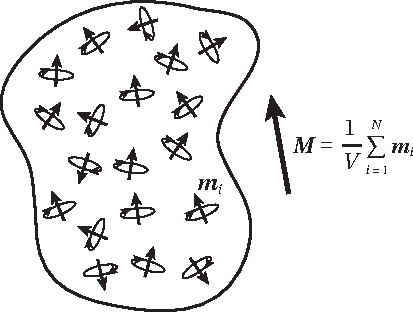
\includegraphics[]{magnetics/figures/magnetization.pdf}
    \caption{Magnetization is the sum of all magnetic moments within a body that give rise to an average magnetization. Magnetization is analogous to density for mass, except that it is a vector quantity.}
    \label{fig:magnetization}
\end{figure}

\subsection{The $B$-field and $H$-field}

There are two quantities that are often referred to as the magnetic field, $\vb{B}$ and $\vb{H}$. We will discuss their relationship shortly, but it is useful to clarify the terminology first, as it can be a source of confusion even among practitioners.

Historically, both $\vb{B}$ and $\vb{H}$ have been called the magnetic field. However, in most geophysical contexts, $\vb{B}$ is what is meant. The quantity $\vb{B}$ is also referred to as the \emph{magnetic induction} or \emph{magnetic flux density}, while $\vb{H}$ is known as the \emph{magnetic field strength} or \emph{magnetic field intensity} \citep{Purcell1985}.

In this chapter, unless otherwise noted, we will use the term \emph{magnetic field} to refer to $\vb{B}$, as this is the quantity that is measured in magnetic surveys. The field $\vb{H}$ will be introduced as the applied or ambient field used to describe how materials become magnetized. While their names may lead to confusion, their physical meanings are quite distinct. The definition of each of these fields is as follows:
\begin{description}
    \item [magnetic flux density, $\vb{B}$,] represents the total magnetic field, including contributions from both external sources and magnetized materials; and
    \item [magnetic field intensity, $\vb{H}$,] represents the applied or ambient magnetic field that drives the magnetization of materials.
\end{description}
In geophysical applications, $\vb{B}$ is the observable quantity, while $\vb{H}$ is used to describe how materials become magnetized.

The two fields are related by
\begin{equation}
    \vb{B} = \mu_0 (\vb{H} + \vb{M}),
\end{equation}
or equivalently,
\begin{equation}
    \vb{H} = \frac{1}{\mu_0}\vb{B} - \vb{M}.
\end{equation}
This relationship shows that the presence of magnetic materials modifies the total magnetic field.

\subsection{Induced magnetization (primary approximation)}

In many geological situations, the magnetization of a material is approximately proportional to the ambient magnetic field,
\begin{equation}
    \vb{M} = \chi \vb{H},
    \label{eq-sus}
\end{equation}
where $\chi$ is the (dimensionless) magnetic susceptibility introduced in the previous section.

Here, $\vb{H}$ represents the Earth's magnetic field, which has a typical magnitude of order $10^4$--$10^5$ \si{A.m^{-1}}. This observation implies that induced magnetization is controlled directly by susceptibility and the strength of the ambient field.

Substituting Equation~\ref{eq-sus} into the previous expression gives
\begin{equation}
    \vb{B} = \mu_0 (1+\chi)\vb{H} = \mu \vb{H},
\end{equation}
where $\mu = \mu_0 (1+\chi)$ is the magnetic permeability.

For most geological materials, $\chi \ll 1$, so $\mu \approx \mu_0$. As a result, variations in magnetic fields are controlled primarily by magnetization rather than changes in permeability.

Under the induced magnetization approximation:
\begin{itemize}
    \item magnetization is aligned with the Earth's magnetic field,
    \item its magnitude is proportional to susceptibility,
    \item anomaly geometry is controlled mainly by the shape of the source.
\end{itemize}
This approximation is the standard assumption used in many magnetic interpretations and forward models.

\subsection{Remanent magnetization (limitations of the approximation)}

In addition to induced magnetization, rocks may carry a remanent magnetization that reflects a past magnetic field. In general,
\begin{equation}
    \vb{M} = \vb{M}_{\mathrm{induced}} + \vb{M}_{\mathrm{remanent}}.
\end{equation}

Remanent magnetization may differ in both magnitude and direction from the present-day Earth's field. When it is significant, it can produce anomalies that deviate from the induced-only assumption.  In particular:
\begin{itemize}
    \item anomaly maxima may be displaced from the source,
    \item anomaly shapes may become asymmetric,
    \item transformations such as reduction to the pole may be inaccurate.
\end{itemize}

Despite these limitations, induced magnetization is often assumed as a first-order approximation. The origin and stability of remanent magnetization will be discussed in detail in the Paleomagnetism (Chapter~\ref{ch:paleomag}).  In practice, this is why magnetic modelling and inversion are commonly expressed in terms of susceptibility rather than magnetization, even though magnetization is the quantity that directly generates the magnetic field.


\section{Magnetic Properties of Rocks and Minerals}

Magnetic anomalies differ from gravity anomalies in one crucial respect: the sources are not ubiquitous. Most rocks contain little magnetic material, and the magnetic response is often controlled by trace amounts of specific minerals. As a result, magnetic anomalies are highly sensitive to mineralogy and alteration rather than bulk composition.

In this chapter, we will primarily assume that magnetization is induced and aligned with the Earth's magnetic field. This assumption greatly simplifies interpretation and is often reasonable, but it is not always valid. We will return to its limitations in later sections and in the Paleomagnetism chapter.

\subsection{Magnetic minerals and trace-element control}

The elements iron (Fe), nickel (Ni), and cobalt (Co) are magnetic, as are many of their oxides.  Iron oxides are the dominant source of magnetism, whereas Ni and Co are generally negligible because they are often orders of magnitude less abundant than Fe.  However, ores of Ni, and Co as well as in mafic and ultramafic rocks high in olivine, serpentinized peridotites, and komatiites may be sufficiently high in Ni that it contributes to the bulk magnetism, though still generally less than Fe.

In most crustal rocks, iron oxides, particularly iron--titanium oxides are the dominant magnetic minerals because they are widely distributed and exhibit a broad range of magnetic behaviours (Figure~\ref{fig:fetiox}).

Fe--Ti oxide minerals form solid-solution series, most importantly:
\begin{itemize}
    \item titanomagnetite, the magnetite--ulv\"ospinel series, and
    \item titanohematite, the hematite--ilmenite series.
\end{itemize}
Magnetic properties vary continuously along these series. For example, increasing Ti content in magnetite reduces both magnetization and Curie temperature. Consequently, even small compositional variations can strongly influence the magnetic behaviour of a rock.
\begin{figure}[hbt]
    \centerline{
        
\includegraphics[]{magnetics/figures/Fe_Ti_oxide_ternary.eps}
    }
    \caption{Compositions of common Fe--Ti oxides with solid solutions and the variations in Curie temperature with composition.}
    \label{fig:fetiox}
\end{figure}

An important geological example is provided by oceanic crust. Basalt formed at mid-ocean ridges commonly contains titanomagnetite, which is the primary carrier of magnetization in the oceanic lithosphere. As these rocks cool, they acquire a remanent magnetization aligned with the Earth's magnetic field at that time. This process is responsible for the linear magnetic anomaly patterns observed on the seafloor (discussed further in Chapter~\ref{ch:paleomag}).

Magnetic mineralogy can also be strongly modified by alteration. For example, at subduction zones and along oceanic faults, hydrothermal alteration of ultramafic rocks (serpentinization) can produce significant quantities of magnetite. This process can enhance magnetic anomalies in regions that would otherwise be only weakly magnetic.

In continental crust, magnetite and hematite are the dominant magnetic minerals. Their relative abundance depends strongly on the oxidation state of the crust. Magnetite typically dominates under reducing conditions, whereas hematite becomes more stable under oxidizing conditions, particularly in the middle and lower crust. This variation influences both the strength and character of magnetic anomalies in continental settings.

These minerals are generally in low abundance.  Hence, magnetic properties are often controlled by accessory mineral phases. A rock containing a small amount of magnetite may produce a stronger magnetic response than a rock composed primarily of weakly and non-magnetic minerals.

\subsection{Magnetic behaviour and susceptibility}

There is no universal mixing law for susceptibility because it depends not only on mineral proportions, but also on grain size, shape, and crystallographic orientation. As a result, susceptibility can vary by many orders of magnitude, even within a single rock type.

Magnetic susceptibility ($\chi$) describes how strongly a material becomes magnetized in response to an applied magnetic field.  It is a bulk property of rocks, but unlike density, susceptibility is not a universal property of matter and can vary over many orders of magnitude.  Materials can be classified according by their magnetic behaviour:
\begin{itemize}
    \item \textbf{Diamagnetic}: very weak, negative susceptibility (e.g., quartz, salt).
    \item \textbf{Paramagnetic}: small, positive susceptibility (common in many silicates).
    \item \textbf{(Ferri)magnetic}: large susceptibility and strong magnetization (e.g., magnetite, pyrrhotite).
\end{itemize}
In most rocks, diamagnetic and paramagnetic contributions are small. The bulk susceptibility is therefore dominated by ferrimagnetic minerals, even when they are present only in trace amounts.

At greater depths, the Earth's mantle is composed primarily of silicate minerals such as olivine and pyroxene, which are paramagnetic. As a result, the mantle contributes only weakly to magnetic anomalies. Most observed crustal-scale magnetic signals therefore originate within the crust, where ferrimagnetic minerals are present.

Representative values of susceptibility for common rocks and minerals are given in Table~\ref{tab-chi}.
\begin{table}
    \centering
    \begin{threeparttable}
    \caption{Table of rock and mineral susceptibilities.}
    \label{tab-chi}
    \begin{tabular}{lc}
        \toprule
        \textbf{Rock Type} & 
        \textbf{Susceptibility Range} \\
        \midrule
        dolomite (pure)   & -12.5 to +44 \\
        dolomite (impure) & 20000 \\
        limestone         & 10 to 25000 \\
        sandstone         & 0 to 21000  \\
        shale             & 60 to 18600 \\
        schist            & 315 to 3000 \\
        slate             & 0 to 38000 \\
        gneiss            & 125 to 25000 \\
        serpentenite      & 3100 to 75000 \\
        rhyolite          & 250 to 37700 \\
        granite           & 10 to 65 \\
        granite (w/ magnetite) & 20 to 50000 \\
        pegmatite         & 3000 to 75000 \\
        basalt            & 500 to 182000 \\
        gabbro            & 800 to 76000 \\
        peridotite        & 95500 to 196000 \\
        hematite          & 420 to 38000 \\
        magnetite         & 70000 to $2 \times 10^{7}$ \\
        ilmenite          & 314000 to $3.8 \times 10^{6}$ \\
        pyrite            & 50 to 5000 \\
        pyrrhotite        & 1250 to $6.3 \times 10^{6}$ \\
        chalcopyrite      & 400 \\
        ice               & -9 \\
        salt              & -10 \\
        graphite          & -80 to -200 \\
        \bottomrule
    \end{tabular}
    \begin{tablenotes}
        \item From \citet{Reynolds1997} pg. 127.
    \end{tablenotes}
    \end{threeparttable}
\end{table}
Several important observations follow:
\begin{itemize}
    \item Susceptibility can be zero or even negative (diamagnetic materials such as salt or ice).
    \item Variability within a rock type often exceeds differences between rock types.
    \item Small amounts of highly magnetic minerals (e.g., magnetite) dominate bulk behaviour.
\end{itemize}

A key implication is that magnetics is often controlled by accessory minerals. A granite containing a fraction of a percent of magnetite may produce a stronger anomaly than a mafic rock lacking magnetite.  Because few minerals are magnetic and those that are, are found in trace amounts.  

Chemical alteration further modifies magnetic properties. Processes such as oxidation, exsolution, and serpentinization can create or destroy magnetic minerals. The formation of magnetite during hydrothermal alteration of oceanic mantle (serpentinization) can enhance magnetic anomalies, 
\[
    6\underbrace{\ce{(Mg,Fe)2SiO4}}_{\text{olivine}} + 7\ce{H2O} \rightarrow
    3\underbrace{\ce{(Mg,Fe)3(Si_2O_5(OH))4}}_{\text{serpentine}} +
    \underbrace{\ce{Fe3O4}}_{\text{magnetite}} + \ce{H2} .
\]
Another example includes the exsolution of titanomagnetite during cooling can change magnetic minerals,
\[
    \underbrace{\ce{Fe_{3-x}Ti_xO4}}_{\text{titanomagnetite}} \rightarrow
    \underbrace{\ce{Fe3O4}}_{\text{magnetite}} +
    \underbrace{\ce{FeTiO3}}_{\text{ilmenite}} + \text{intermediate~spinels} .
\]
Near earth's surface, oxidation to hematite may weaken or modify magnetic signals
\[
    4\underbrace{\ce{Fe3O4}}_{\text{magnetite}} + \ce{O2} \rightarrow
    6\underbrace{\ce{Fe2O3}}_{\text{hematite}} .
\]
Because of this sensitivity, magnetic data are often used as a proxy for alteration patterns, particularly in mineral exploration.

\subsection{Curie temperature}

Magnetic minerals can sustain spontaneous magnetization only below a critical temperature known as the \emph{Curie temperature} ($T_C$). Above this temperature, thermal agitation disrupts magnetic ordering and the material becomes paramagnetic, losing any permanent magnetization.  Curie temperature is therefore a fundamental property that determines whether a mineral can carry a magnetic signal.  Representative values for common magnetic minerals are given in Table~\ref{tab-curie}.
\begin{table}
    \centering
    \begin{threeparttable}
    \caption{Table of common magnetic minerals and Curie temperature.}
    \label{tab-curie}
    \begin{tabular}{lcc}
        \toprule
        Mineral &
        Composition & 
        $T_{\si{C}}$ (\si{^\circ C}) \\
        \midrule
        iron            & $\alpha$\ce{Fe}          & 765 \\
        magnetite       & \ce{Fe3O4}               & 580 \\
        hematite        & $\alpha$\ce{Fe2O3}       & 675 \\
        maghemite       & $\gamma$\ce{Fe2O3}       & 590 to 675 \\
        titanomagnetite & \ce{Fe2.7Ti0.3O4}        & 350 \\
        {}              & \ce{Fe2.4Ti0.6O4}        & 150 \\
        goethite        & $\alpha$\ce{FeO(OH)}     & 120 \\
        pyrrhotite      & \ce{Fe7S8}               & 320 \\
        greigite        & \ce{Fe3S4}               & $\sim$330 \\
        \bottomrule
    \end{tabular}
    \begin{tablenotes}
        \item From {\citet{Dunlop&Ozdemir1997}} p. 51.
    \end{tablenotes}
    \end{threeparttable}
\end{table}

Curie temperature varies significantly between minerals and within mineral series. For example, titanomagnetite shows a strong decrease in $T_C$ with increasing titanium content, consistent with Figure~\ref{fig:fetiox}.  From a magnetic perspective, heating a rock above its Curie temperature will erase any prior magnetization. Upon cooling, the rock may acquire a new magnetization depending on the magnetic field at that time.

We will later return to the implications of Curie temperature at the crustal scale, where it provides a link between magnetic data and temperature structure.

\subsection{Induced and remanent magnetization (conceptual overview)}

There are two sources of magnetization: (1) induced magnetization is proportional to the present-day Earth's magnetic field and is controlled by susceptibility; and (2) remanent magnetization reflects a magnetic field that existed in the past and is retained by the rock.  The total magnetization of a rock can be expressed as the sum of these components,
\begin{equation}
    \coreeq
    \mathbf{M} = \mathbf{M}_{\mathrm{induced}} + \mathbf{M}_{\mathrm{remanent}}.
\end{equation}

In many magnetic surveys, it is assumed that induced magnetization dominates and is aligned with the Earth's field. This approximation simplifies interpretation and underlies many standard processing methods. However, this is not always accurate.

The total magnetization of a rock is the sum of induced and remanent components. The relative importance of these is commonly expressed using the K\"onigsberger ratio,
\begin{equation}
Q = \frac{|\mathbf{M}_{\mathrm{remanent}}|}{|\mathbf{M}_{\mathrm{induced}}|}.
\end{equation}
Typical values include:
\begin{itemize}
    \item $Q < 1$: sedimentary and many metamorphic rocks,
    \item $Q \approx 1$: slowly cooled igneous and regional metamorphic rocks,
    \item $Q \sim 10$: volcanic rocks,
    \item $Q \sim 30$--40: rapidly quenched basalts (e.g., oceanic crust).
\end{itemize}

Many of these minerals can acquire a permanent magnetization that is retained so long as the temperature remains below the Curie temperature. Above $T_C$, thermal agitation destroys long-range magnetic ordering and the material becomes paramagnetic.

For magnetic surveys, the details of how remanent magnetization is acquired are usually less important than its magnitude and direction.  When $Q$ is large, remanent magnetization may dominate the observed anomaly and produce directions that differ significantly from the Earth's present-day field.  This is one of the primary sources of ambiguity in magnetic interpretation and will be revisited later.

The origin and stability of remanent magnetization are central topics in paleomagnetism and will be discussed in detail in the Paleomagnetics chapter (Chapter~\ref{ch:paleomag}).



5. Magnetic Sources and Canonical Models
This parallels gravity, but with a clear warning label.
5.1 Dipoles and prisms
- Direction matters
- Source-anomaly offset
- Comparison to gravity bodies
- Mostly as-is
5.2 Geometry vs direction
- Why magnetics is harder to “eyeball”
- Latitude dependence
- Non-intuitive anomaly shapes
- New interpretive emphasis

\section{Theory}

\subsection{Monopole versus Dipole}

In our discussion on gravity, we described the potential due to mass.  We only have positive masses which create gravitational fields.  The fields are always directed towards the center of mass and are radially symmetric.  As a result, the equipotential surfaces form spheres about the source.  This behaviour can be described as a monopole.

In magnetism, however, monopoles do not exist (at least so far as we currently know---the search goes on).  The processes which generate magnetic fields result in dipolar fields: fields that are axially symmetric (symmetric about a single axis), but vary with orientation.  An example of monopole and dipole fields are shown in Fig.~\ref{fig:poles}. So, unlike gravity, magnetics introduces an additional complexity: the direction of magnetization plays a fundamental role in determining the observed field.

\begin{figure}[hbt]
    \centering
    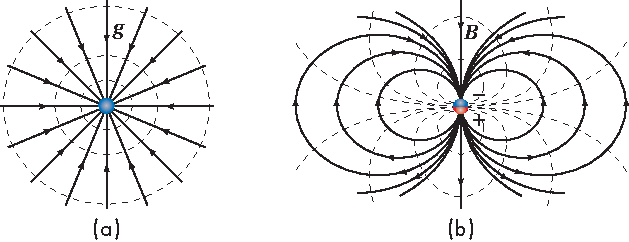
\includegraphics[]{magnetics/figures/poles.pdf}
    \caption{Field lines (solid) and equipotential surfaces (dashed) due to a (a) monopole and (b) dipole.}
    \label{fig:poles}
\end{figure}

This distinction is fundamental for interpretation. In gravity, anomaly shapes are largely controlled by geometry. In magnetics, the dipolar nature of the field introduces an additional dependence on direction, which makes anomaly shapes more complex and less intuitive.

\subsection{Dipolar Field}

\subsubsection{Magnetic Potential}

There are multiple ways to derive the field due to a dipole. One involves modeling two current loops, and while more technically accurate, it is more cumbersome. A simpler conceptual approach is to consider two monopoles of equal and opposite sign separated by a small distance. Although magnetic monopoles are a useful conceptual tool, the fundamental source of magnetic fields is the dipole. A dipole may be viewed as two equal and opposite poles separated by a small distance (Figure~\ref{fig:dipole}), or equivalently as a small current loop.

Using superposition,
\begin{equation*}
    V(P) = V_1(P) + V_2(P),
\end{equation*}
we examine two monopoles of opposite sign and separated by a small distance, $\Delta z$ (Fig.~\ref{fig:dipole}),
\begin{equation*}
    V(P) = -[V_1(P + \Delta z) - V_1(P)] .
\end{equation*}

\begin{figure}[hbt]
    \centering
    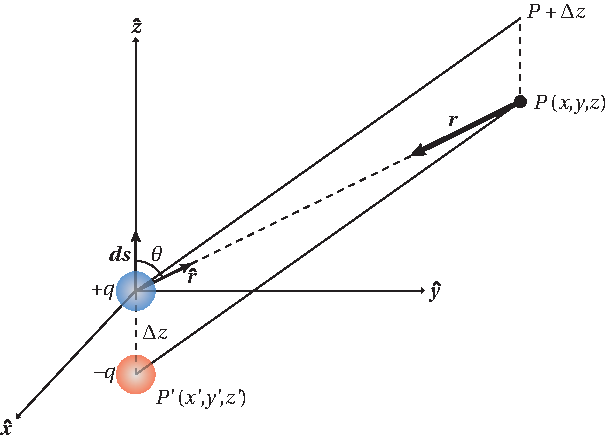
\includegraphics[]{magnetics/figures/two_poles.pdf}
    \caption{Two monopoles of opposite sign in proximity result in a dipolar field. After \citet{Blakely1995}.}
    \label{fig:dipole}
\end{figure}

Taking the limit as the separation becomes small,
\begin{equation*}
    V(P) = - \Delta z \dv{V_1(P)}{z}.
\end{equation*}

Using the magnetic potential of a monopole,
\begin{align}
    U(P) &= G \frac{m}{r} \quad \text{(gravity)} \\
    V_1(P) &= \frac{\mu_0}{4 \pi} \frac{q}{r} \quad \text{(magnetics)},
\end{align}
we obtain
\begin{equation*}
    V(P) = - \frac{\mu_0}{4 \pi} q \Delta z \dv{}{z} \frac{1}{r}.
\end{equation*}

Generalizing to arbitrary orientation,
\begin{equation*}
    V(P) = - \frac{\mu_0}{4 \pi} q \dd{\vb{s}} \cdot \grad \frac{1}{r}.
\end{equation*}

Defining the dipole moment,
\begin{equation}
    \vb{m} = q \dd{\vb{s}},
\end{equation}
gives
\begin{equation}
    V(P) = -\frac{\mu_0}{4 \pi} \vb{m} \cdot \grad \frac{1}{r}.
\end{equation}

\subsubsection{Magnetic Field}

The magnetic field is obtained from the potential,
\begin{equation}
    \vb{B} = - \grad V.
\end{equation}

Applying the vector identity yields
\begin{equation}
    \vb{B}(r,\theta) = \frac{\mu_0}{4 \pi} \frac{m}{r^3}
    [3(\hat{\vb{m}} \cdot \hat{\vb{r}})\hat{\vb{r}} - \hat{\vb{m}}].
\end{equation}

This expression highlights two important features:

\begin{itemize}
    \item The field decays as $1/r^3$, more rapidly than gravity ($1/r^2$).
    \item The field depends explicitly on the orientation of the dipole.
\end{itemize}

The second point is particularly important: unlike gravity, the direction of the source affects the shape of the observed anomaly.

\subsection{From Dipoles to Magnetized Bodies}

Magnetized geologic bodies, while more complex in geometry, can be viewed as a collection of dipoles.  Taking an approach similar to gravity where we reformulated the equations to use density instead of mass, we will view bodies in terms of magnetization instead of dipole moments.  For a material with uniform magnetization $\vb{M}$, each small volume element behaves like a dipole with moment $\vb{m} = \vb{M} \dd{v}$.

Integrating over the body gives
\begin{equation}
    \vb{B} = - \frac{\mu_{0}}{4\pi} \nabla_{P} \int_{V} 
    \vb{M}(Q) \cdot \nabla_{Q} \frac{1}{r} \dd{v}.
    \label{eq-mag}
\end{equation}

While analogous to the gravitational field equation, the vector nature of magnetization with both magnitude and direction influence the magnetic field.

\subsection{Constitutive Relationship and Poisson Analogy}

In the induced magnetization approximation,
\begin{equation}
    \vb{M} = \chi \vb{H}.
\end{equation}

Substituting this into Equation~\ref{eq-mag} shows that the magnetic field is controlled by the spatial distribution of susceptibility, much like density in gravity.

The magnetic potential satisfies a Poisson-type equation,
\begin{equation}
    \laplacian V = \div \vb{M}.
\end{equation}

Under induced magnetization,
\begin{equation}
    \laplacian V = \div (\chi \vb{H}),
\end{equation}
which demonstrates that magnetic anomalies arise from spatial variations in susceptibility and from the direction of the inducing field.

This is a key distinction from gravity: even when susceptibility is the parameter being modeled, the resulting field depends on both geometry and field direction.

\subsection{Conceptual Representations of Magnetic Fields}

There are three equivalent conceptual models:

\begin{enumerate}
    \item Magnetic poles
    \item Current loops
    \item Uniformly magnetized bodies
\end{enumerate}

\begin{figure}[hbt]
  \centering
  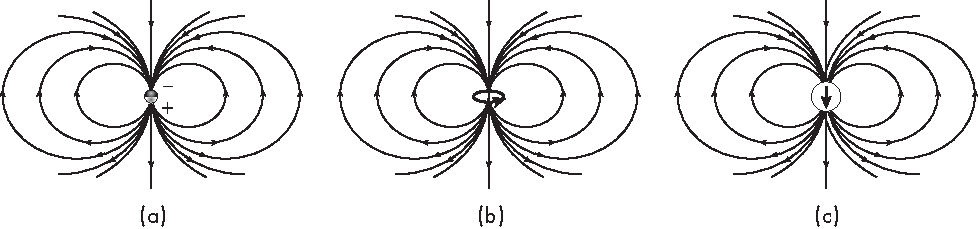
\includegraphics[]{magnetics/figures/magnetic_fields.pdf}
  \caption{Conceptual representations of magnetic fields.}
  \label{fig:magfields}
\end{figure}

These representations all produce equivalent dipole fields and are used interchangeably.

\subsection{Geometry versus Direction}

In gravity, anomaly shapes are largely controlled by source geometry. In magnetics, both geometry and direction matter.  And while all magnetic models reduce to dipoles at sufficient distance, the observable anomalies differ strongly from gravity.

As shown in Fig.~\ref{fig:monodi},
\begin{figure}[hbt]
  \centerline{
    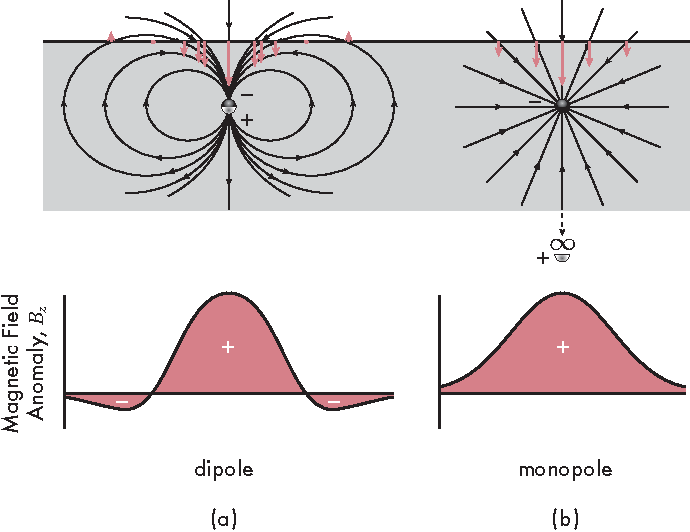
\includegraphics[]{magnetics/figures/monodipole.pdf}
  }
  \caption{Dipole versus monopole responses.}
  \label{fig:monodi}
\end{figure}

\begin{itemize}
    \item Magnetic anomalies are typically asymmetric.
    \item The anomaly peak is often offset from the source.
    \item The anomaly shape depends on the direction of the Earth's field (i.e., latitude).
\end{itemize}

This directional dependence makes magnetic anomalies significantly more difficult to interpret by inspection than gravity anomalies.

\emph{Key point:} Magnetic anomalies are controlled by both the geometry of the source and the direction of magnetization. This dual dependence is the primary reason magnetics is less intuitive than gravity.

\ntextbox{Practical perspective}{
    Magnetics is often described as more complex than gravity because magnetization is a vector quantity and anomaly shapes depend on direction. However, this does not necessarily make magnetic modelling more difficult.

    In practice, magnetized bodies are represented using simple geometric elements (e.g., prisms), and their fields are computed by superposition, just as in gravity. Once the direction of magnetization is specified or approximated (for example, using reduction to the pole), magnetic modelling becomes comparable in complexity to gravity modelling.

    Magnetics also has two important advantages for exploration:
    \begin{itemize}
        \item Magnetic anomalies are largely confined to the crust because most mantle temperatures exceed the Curie temperature.
        \item Magnetic fields decay more rapidly with distance ($B \propto 1/r^3$) than gravitational fields ($g \propto 1/r^2$), producing sharper anomalies for the same source.
    \end{itemize}
}{core}\label{box:mag_adv}

\subsection{Magnetic Field of a Rectangular Prism}

A rectangular prism with uniform magnetization provides one of the most important canonical models in applied magnetics. It forms the basis for most forward modelling and inversion methods, where complex bodies are represented as collections of simple elements.

Consider a rectangular prism bounded by
\[
x_1 \le x \le x_2,\quad
y_1 \le y \le y_2,\quad
z_1 \le z \le z_2,
\]
with observation point at $(x,y,z)$ and magnetization $\vb{M} = (M_x, M_y, M_z)$.

Define shifted coordinates
\[
X_i = x - x_i,\quad 
Y_j = y - y_j,\quad 
Z_k = z - z_k,
\]
where $i,j,k \in \{1,2\}$.

Also define
\[
r_{ijk} = \sqrt{X_i^2 + Y_j^2 + Z_k^2}.
\]

The magnetic field components can be written as

\begin{align}
B_x &= \frac{\mu_0}{4\pi} \sum_{i,j,k} (-1)^{i+j+k}
\bigg[
M_x \tan^{-1}\left( \frac{Y_j Z_k}{X_i r_{ijk}} \right)
- M_y \ln (r_{ijk} + Z_k)
- M_z \ln (r_{ijk} + Y_j)
\bigg],
\\
B_y &= \frac{\mu_0}{4\pi} \sum_{i,j,k} (-1)^{i+j+k}
\bigg[
M_y \tan^{-1}\left( \frac{X_i Z_k}{Y_j r_{ijk}} \right)
- M_x \ln (r_{ijk} + Z_k)
- M_z \ln (r_{ijk} + X_i)
\bigg],
\\
B_z &= \frac{\mu_0}{4\pi} \sum_{i,j,k} (-1)^{i+j+k}
\bigg[
M_z \tan^{-1}\left( \frac{X_i Y_j}{Z_k r_{ijk}} \right)
- M_x \ln (r_{ijk} + Y_j)
- M_y \ln (r_{ijk} + X_i)
\bigg].
\end{align}

These expressions show that the magnetic field is computed as a sum over the eight corners of the prism, with alternating signs. This structure is analogous to the Talwani formulation for gravity, where the field is expressed in terms of contributions from the corners of a polygon.

The logarithmic and arctangent terms arise from the integration of dipole contributions over the volume of the body.

Care must be taken in evaluating the logarithmic and arctangent terms near singularities (e.g., when $X_i$, $Y_j$, or $Z_k$ approach zero). In practice, stable numerical implementations use the two-argument arctangent function and avoid evaluating expressions exactly on prism boundaries.

A key distinction from gravity is that the magnetic field depends explicitly on the components of the magnetization vector $(M_x, M_y, M_z)$. As a result:
\begin{itemize}
    \item both geometry and direction control the anomaly,
    \item changing magnetization direction can strongly alter anomaly shape,
    \item identical bodies can produce very different anomalies depending on magnetization.
\end{itemize}

Under the induced magnetization assumption,
\begin{equation}
    \vb{M} = \chi \vb{H}_0,
\end{equation}
where $\vb{H}_0$ is the Earth's magnetic field.

In this case, the direction of $\vb{M}$ is known, and the problem reduces to determining the effect of the prism geometry and susceptibility.

This represents a first-order approximation. If remanent magnetization is significant, the direction of $\vb{M}$ must be specified independently.

Although these expressions appear more complex than their gravity equivalents, they are straightforward to evaluate numerically. In practice, complex bodies are modeled by dividing the subsurface into many prisms and summing their contributions.

Under simplifying assumptions such as induced magnetization or reduction-to-the-pole, magnetic modelling becomes comparable in difficulty to gravity modelling.


\section{Intuitive Field Shapes and Source Geometry}

The formal development of magnetic fields in the previous section provides a complete mathematical description of magnetic sources. However, interpretation often relies on developing an intuitive understanding of how different source geometries produce characteristic anomaly shapes.

In this section, we examine simplified bodies and build intuition by viewing magnetized objects as collections---\emph{superposition}---of dipoles. This perspective allows us to anticipate the qualitative form of magnetic anomalies without performing detailed calculations.

\subsection{A narrow, vertically magnetized dike}

Consider a narrow vertical dike with uniform magnetization directed vertically. If the width of the dike is small compared to its depth extent, the body behaves approximately as a single dipole.

In this case:
\begin{itemize}
    \item the anomaly is symmetric about the center of the body,
    \item a single peak (or trough) is observed,
    \item the anomaly resembles the response of an isolated dipole.
\end{itemize}

As the depth extent of the dike increases, the anomaly becomes increasingly dipole-like. This reflects the fact that the distant portions of the body contribute less strongly to the field, and the response is dominated by the bulk moment of the source.

\subsection{A wide dike or sill: superposition of dipoles}

Now consider increasing the width of the dike (or equivalently, a sill). The body can be viewed as a collection of dipoles distributed along a horizontal line.

To understand the resulting anomaly, consider the vertical component of the magnetic field, $B_z$, at different observation points.

\paragraph{Observation above the center}

At a point directly above the center of the body:

\begin{itemize}
    \item the dipole directly beneath the observation point contributes the largest positive $B_z$,
    \item nearby dipoles also contribute positively, but less strongly because their field lines spread outward and include horizontal components,
    \item dipoles further away eventually contribute negatively, as their field lines intersect the observation point from below at an opposing orientation.
\end{itemize}

The combined effect is a relatively high value of $B_z$ at the center, but lower than the peak values observed near the edges of the body due to the influence of these distant negative contributions.

\paragraph{Observation near the edge}

At a point near the edge of the body:

\begin{itemize}
    \item dipoles to one side of the observation point contribute positively,
    \item dipoles on the opposite side include both positive and negative contributions, but the geometry results in a net enhancement,
    \item the balance of contributions leads to a maximum in $B_z$ near the edge of the body.
\end{itemize}

\paragraph{Observation beyond the edge}

Beyond the edge of the body:

\begin{itemize}
    \item only dipoles on one side contribute,
    \item these contributions become increasingly negative with distance,
    \item the field decays toward zero from the negative side.
\end{itemize}

This behaviour is mirrored on both sides of the body, resulting in a symmetric anomaly with:
\begin{itemize}
    \item peaks near the edges,
    \item a lower-amplitude plateau over the center,
    \item decay to zero at large distances.
\end{itemize}

\subsection{Summary: width and depth effects}

From these examples, several general principles emerge:

\begin{itemize}
    \item Increasing depth extent makes a body appear more dipole-like.
    \item Increasing lateral extent produces broader anomalies with edge enhancements.
    \item The observed field at any point is the result of competing positive and negative contributions from different parts of the source.
\end{itemize}

These effects are a direct consequence of the dipolar nature of magnetic fields.

\subsection{Effect of magnetization direction}

The examples above assumed vertical magnetization. If the direction of magnetization is changed, the relative contributions from different parts of the body also change.

For a single dipole:
\begin{itemize}
    \item the direction of $\vb{M}$ controls the orientation of the field,
    \item the position of anomaly maxima shifts relative to the source,
    \item the anomaly becomes asymmetric.
\end{itemize}

For extended bodies, this effect is amplified:
\begin{itemize}
    \item peaks shift laterally,
    \item positive and negative lobes become unequal,
    \item anomaly shapes depend strongly on latitude through the Earth's field direction.
\end{itemize}

\noindent {\bf Key observation.} Magnetic anomalies cannot be understood purely in terms of geometry. Even for simple bodies, the distribution of positive and negative contributions depends on both the shape of the source and the direction of magnetization.

\section{Measuring the Magnetic Field}

Magnetic surveys measure the total magnetic field, which includes contributions from both the Earth's main field and local variations caused by magnetized structures in the crust. In practice, the measured field must be corrected to isolate these local variations (deviations), known as magnetic anomalies---the primary target of interpretation.

The Earth's magnetic field is dominated by a large-scale component generated in the core, which varies smoothly in space and time. Superimposed on this are smaller-scale contributions from the crust, which are the focus of magnetic exploration.

Magnetic data processing is generally simpler than gravity because fewer corrections are required. The main steps are:
\begin{itemize}
    \item removal of temporal variations (diurnal correction),
    \item removal of the Earth's main field (IGRF),
    \item optional separation of regional and residual components.
\end{itemize}

\subsection{Magnetometers}

The commonly used varieties in use today are alkali vapor (optically pumped) magnetometers and proton precession magnetometers.  These types can be hand-held, or mounted to a moving vehicle (car, airplane, ship).  Alkali vapor and proton precession magnetometers measure the total magnetic field strength,
\[
T = |\vb{B}|,
\]
but not its direction.

For total field magnetometers, it is common to express anomalies as the projection of the magnetic field onto the direction of the regional field, $\hat{\vb{F}}$. The total field anomaly is then approximated as
\[
    \delta T = \hat{\vb{F}} \cdot \delta \vb{B},
\]
which, using Equation~\ref{eq-mag}, can be written as
\[
    \delta T = - \frac{\mu_{0}}{4\pi} \hat{\vb{F}} \cdot \nabla_{P}
    \int_{V} \vb{M} \cdot \nabla_{Q}
    \frac{1}{r} dv.
\]

Also commonly used for airborne, shipborne, satellite, and base station measurements are flux gate magnetometers.  Flux gates measure the field strength in one direction so they are generally used in combination of three to measure the vector field magnitude in three orientations.  This vector measurement can be highly advantageous as it can aid in interpreting and modeling anomalies.

\subsection{The Earth's main field (IGRF)}

The dominant contribution to the measured magnetic field is the Earth's main field, generated by dynamo processes in the liquid outer core. This field is smooth at the scale of most surveys and varies gradually as a function of latitude, longitude, and time.

The International Geomagnetic Reference Field (IGRF) provides a standard model of the Earth's main field based on spherical harmonic expansions. It is periodically updated to account for secular variation.

The IGRF defines, at any location and time:
\begin{itemize}
    \item the total field strength,
    \item the inclination (dip angle),
    \item the declination (horizontal direction).
\end{itemize}

These parameters are used to define the direction of the inducing field $\vb{H}_0$ in modelling.

\begin{figure}[hbt]
  \centering
  %\includegraphics[]{magnetics/figures/igrf_global.pdf}
  \caption{Global distribution of the Earth's magnetic field strength (IGRF model).}
  \label{fig:igrf}
\end{figure}

\subsubsection{Latitude and Longitude Corrections}

The Earth's main magnetic field is typically removed using a reference model such as the IGRF.  This correction produces the residual field, which isolates contributions from crustal magnetization.

For small surveys, this correction may be approximated by subtracting a constant value or may not be done at all. For larger surveys, a spatially varying reference field is required, adjusting for spatial variations in latitude and longitude.

\subsection{Additional Corrections}

Very few corrections are necessary for magnetic data which makes data reduction significantly simpler than gravity.

\subsubsection{Diurnal Variations}

The Earth's magnetic field is warped by the solar wind, compressing magnetic field lines in the direction of the sun and stretching out the field lines away from the sun (Fig.~\ref{fig:solarwind}).  Additionally, the intensity of the solar wind varies due to normal solar processes causing the magnetic field to pulse as it pushes back.  The intensity of these pulsations and compression of field lines can be particularly large during solar storms.  However, we can account for these variations by continuously recording the magnetic field at a base station somewhere within or nearby the field site.
\begin{figure}[hbt]
  \centerline{
    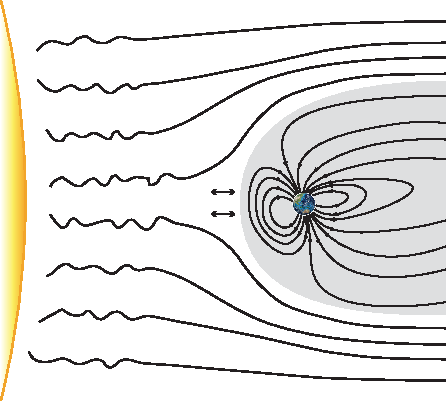
\includegraphics[]{magnetics/figures/solar_wind.pdf}
  }
  \caption{The Earth's magnetic field is distorted by the solar wind.}
  \label{fig:solarwind}
\end{figure}

\subsubsection{Altitude and Topography}

Because the magnetic field varies with height above the Earth's surface, small elevation differences can introduce variations in the measured field. These effects are typically small ($<0.03$~nT~m$^{-1}$) and are often neglected.

However, airborne surveys may be flown at different altitudes above the land surface.  In such cases, surveys can be combined only after adjusting one or both so that they approximate the same flight altitude.  Such adjustements are typically made using upward or downward continuation (Section~\ref{sec:continuation}).

The topographic correction is generally not applied, but may be necessary in some cases with significant topography and highly magnetized terranes (e.g., lava flows and intrusions).

\subsection{Magnetic Anomalies}

As discussed previously, the magnetic field due to a body can be viewed in terms of pole pairs, currents or uniform magnetization.  As seen from the equations for a dipole, the observed magnetic field from a body depends not only upon the distance from the body, but also the azimuth.  In the case of buried structures or targets, the orientation of magnetization may not be purely vertical or horizontal making the observed response asymmetric (Figure~\ref{fig:skew}).
\begin{figure}[hbt]
  \centerline{
    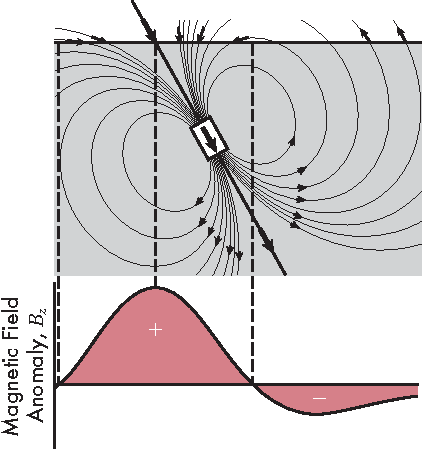
\includegraphics[]{magnetics/figures/skew_dipole.pdf}
  }
  \caption{The vertical component of a rotated dipole that is buried near the surface shows a highly asymmetric response.  Note that the orientation of the survey across the dipole would be different.}
  \label{fig:skew}
\end{figure}
The shape of the body and its extent also affect the observed response (Fig.~\ref{fig:nvw}).
\begin{figure}[hbt]
  \centerline{
    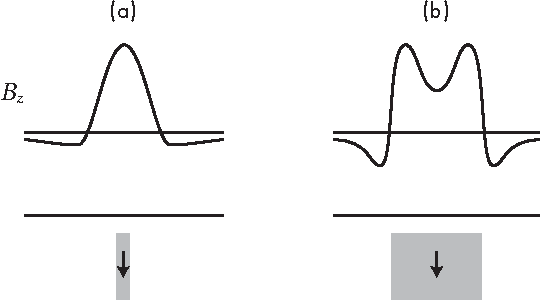
\includegraphics[]{magnetics/figures/narrow_vs_wide.pdf}
  }
  \caption{The vertical magnetic response of a (a) narrow and (b) wide body magnetized in the vertical direction.}
  \label{fig:nvw}
\end{figure}

\section{Regional residuals}

Whereas gravitational attraction results from the density structure of the Earth from the top of the atmosphere to the core, magnetic variations come from the core (Earth's field) and the lithosphere (remnant and induced magnetization).

Regional residuals for magnetics are removed much the same way as they are for gravity.  After removal of the main field (e.g., IGRF), remaining long-wavelength variations may still be present and can be separated using methods similar to those used in gravity.  For example, Upward continuation is commonly used to suppress shallow sources and emphasize regional trends, while downward continuation enhances shallow features but amplifies noise.  Fourier domain filtering is also widely used to separate regional and residual components.

\section{Transformations and Spectral Thinking}

Magnetic anomalies are strongly influenced by the direction of magnetization and the spatial distribution of sources. As a result, raw magnetic data can be difficult to interpret directly. A variety of transformations are therefore used to simplify anomaly shapes, enhance specific features, or extract information about source depth.

Many of these transformations are most naturally expressed in the Fourier domain, where operations such as filtering, differentiation, and continuation become simple algebraic manipulations. In this section, we focus on the physical meaning and practical implications of these transformations, leaving detailed derivations to the Fourier Transform chapter.

\subsection{Reduction to the Pole (RTP)}

The reduction to the pole transform is designed to simplify the interpretation of magnetic anomalies by transforming the observed field to the response that would be measured if both the Earth's magnetic field and the magnetization were vertical (i.e., inclination of $90^\circ$).
\begin{center}
    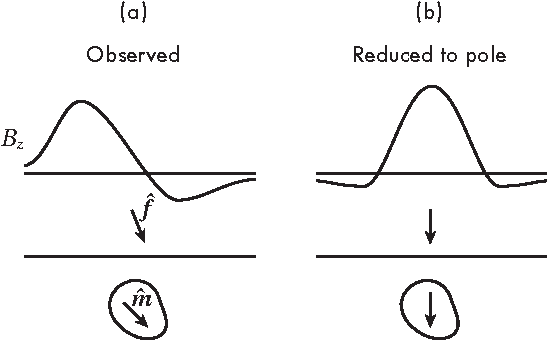
\includegraphics[]{magnetics/figures/reduced_to_pole.pdf}
    \captionof{figure}{The reduction to the pole transforms the observed Earth's field and magnetization orientations, $\vu{f}$ and $\vu{m}$, to the vertical.}
    \label{fig:rtpole}
\end{center}

Physically, the effect of RTP is to remove the directional dependence of the magnetic field. As a result, anomalies become more symmetric and their maxima are shifted closer to the source location. In this sense, RTP transforms magnetic data into something that more closely resembles gravity, where anomaly geometry is easier to interpret.

In the Fourier domain, RTP is implemented as a filter that depends on the direction of the Earth's field and the magnetization. The mathematical expression involves both amplitude and phase modification and is therefore sensitive to noise and numerical instability. (Details are provided in Box~\ref{box:rtp}.)

\ntextbox{Reduction to pole}{
    The reduction to pole transform is meant to simplify interpretation of magnetic maps by transforming the Earth's and magnetized field from the observed to vertical, 90$^\circ$ (Fig.~\ref{fig:rtpole}).
    \begin{center}
        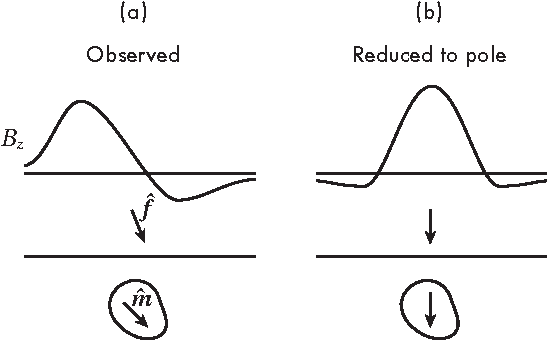
\includegraphics[]{magnetics/figures/reduced_to_pole.pdf}
        \captionof{figure}{The reduction to pole transforms the observed Earth's field and magnetization orientations, $\vu{f}$ and $\vu{m}$, to the vertical.}
        \label{fig:rtpole}
    \end{center}

    The reduction to pole transform is a Fourier domain technique given by
    \[
        \ft{\Delta T_{r}} = \ft{\psi_{r}} \ft{\Delta T},
    \]
    where $\ft{\psi_{r}} = \Theta_{m} \Theta_{f}$ and is related to the direction of magnetization, $\vu{m} = (\vu{m}_x,\vu{m}_y,\vu{m}_z)$, and the Earth's field direction, $\vu{f} = (\vu{f}_x,\vu{f}_y,\vu{f}_z)$, by
    \begin{eqnarray*}
        \Theta_{m} & = & \vu{m}_{z} 
            + i\frac{\vu{m}_x k_x + \vu{m}_y k_y}{|k|}, \\
        \Theta_{f} & = & \vu{f}_{z} 
            + i\frac{\vu{f}_x k_x + \vu{f}_y k_y}{|k|}.
    \end{eqnarray*}
    Both $\vu{m}$ and $\vu{f}$ are unit vectors.

    \noindent {\bf Pros:}
    \begin{itemize}
        \item Often helps identify the source of an anomaly by placing a peak over the center or edges.
    \end{itemize}
    {\bf Cons:}
    \begin{itemize}
        \item Only works when the remnant field is induced (i.e.\ magnetized at the same inclination as the Earth's present-day field).
        \item The transform is unstable at low latitudes ($\pm$10$^\circ$) due to the large rotation of inducing field; although, a mathematical fix is possible in some cases.
    \end{itemize}
}{aside}\label{box:rtp}

RTP performs well when several conditions are satisfied: the magnetization is primarily induced so that $\vb{M} \parallel \vb{H}_0$, the data are acquired at moderate to high magnetic latitudes, and the anomaly geometry is relatively simple.

However, it becomes unreliable when these assumptions break down. In particular:
\begin{itemize}
    \item significant remanent magnetization alters the direction of $\vb{M}$,
    \item low magnetic latitudes require large phase rotations,
    \item noise and limited data extent introduce instability.
\end{itemize}

At low latitudes in particular, the transformation becomes unstable because it requires large phase rotations of the data. Modified or stabilized versions of RTP exist, but care must always be taken in interpreting the results.

\emph{Key idea:} RTP attempts to remove directional complexity from magnetic data. When its assumptions are valid, it can make magnetics look much more like gravity.

\subsection{Continuation and Filtering (Conceptual View)}

Continuation and filtering are often used to emphasize features at different scales or depths.

\paragraph{Depth--wavelength relationship}

A fundamental principle in potential field methods is that:
\begin{center}
\emph{long wavelengths are associated with deeper sources, while short wavelengths are associated with shallow sources.}
\end{center}

This arises from the decay of potential fields with distance (e.g., $B \propto 1/r^3$ for dipoles). In the Fourier domain, this relationship becomes explicit through exponential weighting of different spatial frequencies.

Upward continuation smooths the field by preferentially attenuating short wavelengths. Because these short wavelengths are associated with shallow sources, the resulting field emphasizes deeper, more regional structure.

Downward continuation has the opposite effect, amplifying short-wavelength components and enhancing shallow features. However, this enhancement applies equally to signal and noise, making the process intrinsically unstable. Even small errors in the data can grow rapidly, limiting its practical use.

As a result, downward continuation is inherently unstable and must be used with caution.

\paragraph{Derivative and filtering operations}

All filtering operations involve a trade-off between resolution and stability. Enhancing high-frequency components can sharpen anomalies and improve edge detection, but it also amplifies noise. As a result, the effective resolution of filtered data is often controlled more by noise than by the underlying signal.

In practice, all such operations involve a trade-off between resolution and stability.

\emph{Key idea:} Filtering redistributes energy between spatial scales. Enhancing small features always comes at the cost of increased sensitivity to noise.

\subsection{Pseudo-gravity Transformation}

The pseudo-gravity transform attempts to convert a magnetic anomaly into an equivalent gravity anomaly under simplifying assumptions.

The motivation for this transformation comes from the formal similarity between gravitational and magnetic potentials. If both density and magnetization are constant within a body, the two fields are related through spatial derivatives.

In practice, the transformation is implemented as a Fourier-domain filter that converts the observed magnetic field into a pseudo-gravity response (Box~\ref{box:pseudogravity}).

\ntextbox{Pseudo-gravity}{
The pseudo-gravity transform attempts to take a magnetic anomaly and estimate the gravitational attraction.  If density and magnetization are constant, we can write the gravitational and magnetic potentials as
\begin{eqnarray*}
    U_{g}(P) & = & G \rho\int_{V} r^{-1} dv, \\
    U_{m}(P) & = & - \frac{\mu_0}{4\pi}\vb{M} \cdot \nabla_{P} \int_{V} r^{-1} dv.
\end{eqnarray*}
Note the similarity between the two potentials, we can show that 
\[
    U_{m}(P) = -\frac{\mu_0}{4\pi G \rho} \vb{M} \cdot \nabla_{P} U_{g}.
\]
Recall, $g = \nabla U_{g}$; therefore,
\[
    U_{m}(P) = -\frac{\mu_0 M g_{m}}{4\pi G \rho},
\]
where $g_{m}$ is the component of gravity in the direction of magnetization.  But we really care about the vertical component of $g$ just as we would observe from a gravity survey.  To find this, we have to return to the Fourier domain where it can be shown that
\[
    \ft{\Delta T_{psg}} = \ft{\psi_{psg}} \ft{\Delta T},
\]
where $\Delta T_{psg}$ is the pseudo-gravity derived from the total field and
\[
    \ft{\psi_{psg}} = \frac{4\pi G}{\mu_{0} |k| \Theta_{m} \Theta_{f}} \frac{\rho}{M}.
\]
The psuedo-gravity transform in this way is related to the reduction to pole shown earlier (i.e.\ $\ft{\psi_{psg}} = 4\pi G \mu_{0}^{-1} |k|^{-1} \ft{\psi_{r}}$).  As a result, the pseudo-gravity transform also suffers from numerical instability at low latitudes.

There is also a pseudo-magnetic transform that can be applied to observed gravity.  However, the pseudo-magnetic transformation can be unstable and is basically never used anyway.
}{aside}\label{box:pseudogravity}

The pseudo-gravity transform can provide a more intuitive representation of magnetic data because gravity anomalies are often easier to interpret geometrically. By reducing directional effects, the transform produces responses that resemble those of density variations, highlighting the density-like behaviour of magnetic sources and aiding qualitative interpretation.

These advantages must be balanced against important limitations. The transformation assumes a constant ratio of magnetization to density ($M/\rho$), which is rarely satisfied in heterogeneous crustal environments. It is also sensitive to errors in the assumed magnetization direction, and shares the same instability issues as reduction to the pole, particularly at low magnetic latitudes. As a result, pseudo-gravity is best used as a qualitative interpretive tool rather than a quantitative inversion method.

As a result, pseudo-gravity is best viewed as an interpretive aid rather than a quantitative transformation.

\subsection{Curie Depth (Spectral Perspective)}


Because most mantle minerals are paramagnetic and crustal minerals lose magnetization at elevated temperatures, the ability of the Earth to generate magnetic anomalies is largely restricted to relatively shallow regions containing ferrimagnetic minerals below the Curie temperature.

This depth can be estimated using spectral methods by examining the longest wavelengths present in the data. Under the assumption that deeper sources produce longer wavelengths, the low-wavenumber content of the magnetic field provides an estimate of the maximum depth of magnetization.

If we know the mineral the mineral responsible for the majority of magnetization of the crust, then we can assign a temperature to this depth based on the Curie temperature (Table~\ref{tab-curie}).  Identifying the variations in depth of this Curie isotherm allows us to estimate surface heat flow and geotherms.  While this may not be useful for small studies, it may be useful for identifying possible geothermal targets on a regional basis\ldots though in my experience the results do not match surface heat flow estimates all that well and should be used with caution.

Estimates of Curie depth provide a measure of the base of the magnetized crust. Where the dominant magnetic mineral is known, this depth can be related to thermal structure through its Curie temperature, offering insight into subsurface temperature distributions. As a result, Curie depth estimates are most useful at regional scales, where they can help identify large-scale thermal variations such as those associated with geothermal systems.

These interpretations rely on several simplifying assumptions. In particular, they require that a single magnetic mineral with a known Curie temperature dominates the magnetic signal, which is often not the case in heterogeneous crust. The method also depends on approximate relationships between wavelength and depth, introducing additional uncertainty. Furthermore, spectral estimates are sensitive to noise and the spatial extent of the data, which can significantly affect the reliability of the inferred depths.

Thus, Curie depth estimates should be interpreted as approximate and model-dependent.

\subsection{Why Fourier Space Matters (Preview)}

Many of the transformations discussed above are most naturally expressed in the Fourier domain.

In real space:
\begin{itemize}
    \item operations such as continuation or differentiation involve integrals,
    \item directional effects are difficult to isolate.
\end{itemize}

In Fourier space:
\begin{itemize}
    \item convolution becomes multiplication,
    \item derivatives become simple algebraic factors,
    \item directional filters (such as RTP) can be applied directly.
\end{itemize}

This makes Fourier methods computationally efficient and conceptually powerful.

\emph{Key idea:} Fourier space provides a natural framework for manipulating potential fields. Many operations that are complex in real space become simple, intuitive filters in the spectral domain.

\section{Non-Uniqueness and Ambiguity in Magnetics}

All potential field methods are inherently non-unique: many different subsurface models can produce the same observed field. However, magnetics departs from gravity in a fundamental way, as ambiguity arises not only from source geometry, but also from the direction and nature of magnetization.

In gravity, anomalies are controlled primarily by the geometry of density contrasts. In magnetics, the situation is more complex because magnetization is a vector quantity. A single body may produce very different anomalies depending on the direction of magnetization, leading to asymmetry in anomaly shapes and offsets between anomaly maxima and the true source location. Consequently, different combinations of geometry and magnetization direction can yield similar observed fields, making interpretation by inspection significantly more difficult than in gravity.

A further source of ambiguity arises from the distinction between induced and remanent magnetization. In many applications, it is assumed that magnetization is induced and aligned with the present-day Earth's magnetic field. While this assumption simplifies interpretation, it is not always valid. When remanent magnetization is present and significant, the direction of the total magnetization vector may differ substantially from that of the Earth's field. This can result in anomaly shapes that are inconsistent with induced-only models and can cause transformations such as reduction to the pole to fail or produce misleading results. Because remanent magnetization is often poorly constrained, it is difficult to separate its effects from those of geometry.

Magnetic data are frequently interpreted in terms of susceptibility, particularly under the assumption of induced magnetization. However, the observed field is produced by the total magnetization, not susceptibility alone. This introduces another level of ambiguity. A strong anomaly may reflect high susceptibility, strong remanent magnetization, or some combination of both. Similarly, rocks with low susceptibility may still generate significant anomalies if remanence is large. In practice, different combinations of susceptibility and remanent magnetization can give rise to similar magnetic fields, complicating attempts to infer material properties directly from the data.

Taken together, these factors mean that ambiguity in magnetics arises from both geometry and magnetization. In practice, this requires a more cautious approach to interpretation than in gravity. Multiple models should be considered, underlying assumptions about magnetization should be stated explicitly, and additional constraints—such as geological information, petrophysical measurements, or other geophysical data—are often necessary to reduce uncertainty. Despite these challenges, magnetics remains a powerful tool, particularly because of its sensitivity to small amounts of magnetic minerals. With appropriate assumptions and supporting information, it can provide high-resolution insight into the distribution and history of magnetized materials in the crust.

\emph{Key idea:} Non-uniqueness in magnetics arises from both geometry and magnetization. Unlike gravity, where density is the primary unknown, magnetic interpretation must also account for the magnitude and direction of magnetization.

\section{Forward Modeling Paradigms}

Given the non-uniqueness and ambiguity inherent in magnetic data, interpretation is most commonly carried out through forward modelling. In this approach, a subsurface model is proposed, its magnetic response is computed, and the result is compared with the observed data. The model is then refined iteratively until an acceptable match is obtained.

As in gravity, forward modelling relies on the principle of superposition: the total magnetic field is obtained by summing the contributions from many simple elements. However, because magnetization is a vector quantity, magnetic modelling requires specification not only of material properties and geometry, but also of magnetization direction.

Under the assumption of induced magnetization, we write
\begin{equation}
    \vb{M} = \chi \vb{H}_0,
\end{equation}
so that the direction of $\vb{M}$ is known. In the more general case, the magnetization must be specified explicitly as a vector field,
\begin{equation}
    \vb{M}(\vb{r}) = [M_x(\vb{r}), M_y(\vb{r}), M_z(\vb{r})].
\end{equation}

The forward problem then consists of computing the magnetic field from this distribution of magnetization.

\subsection{Voxel (cell-based) models}

A common approach is to discretize the subsurface into a collection of small volume elements (voxels or pixels), each with uniform magnetization. The total magnetic field is then approximated as a sum over contributions from each cell.

Using the prism formulation introduced earlier, the field at an observation point can be written schematically as
\begin{equation}
    \vb{B}(\vb{r}) = \sum_{n=1}^{N} \mathbf{G}_n(\vb{r}) \, \vb{M}_n,
\end{equation}
where $\mathbf{G}_n$ represents the geometric kernel for voxel $n$, and $\vb{M}_n$ is the magnetization vector of that cell.

For total-field data, the forward model is typically written as
\begin{equation}
    \delta T(\vb{r}) = \vu{F} \cdot \vb{B}(\vb{r})
    = \sum_{n=1}^{N} \vu{F} \cdot \mathbf{G}_n(\vb{r}) \, \vb{M}_n,
\end{equation}
where $\vu{F}$ is the unit vector in the direction of the Earth's field.

In the induced magnetization approximation, this reduces to
\begin{equation}
    \delta T(\vb{r}) = \sum_{n=1}^{N} \vu{F} \cdot \mathbf{G}_n(\vb{r}) \, (\chi_n \vb{H}_0).
\end{equation}

This formulation highlights an important difference from gravity. In gravity, each cell contributes a scalar quantity proportional to density. In magnetics, each cell contributes a vector quantity, increasing the number of parameters and the potential for ambiguity.

As a result, voxel-based models are flexible but often underdetermined. They are used extensively in inversion, where regularization is required to constrain the solution.

\subsection{Equivalent source representations}

An alternative approach is to represent the magnetic field using a distribution of equivalent sources, rather than attempting to model the true geological body directly.

In this method, a set of sources (e.g., dipoles or monopole pairs) is placed on a surface or at a constant depth, and their strengths are adjusted to reproduce the observed field. The forward model can be written as
\begin{equation}
    \delta T(\vb{r}) = \sum_{n=1}^{N} a_n \, G_n(\vb{r}),
\end{equation}
where $a_n$ are the amplitudes of the equivalent sources and $G_n$ are their Green's functions.  A Green's function describes the response of a field to a unit point source, and provides a fundamental building block from which solutions for arbitrary source distributions can be constructed by superposition.

In equivalent source methods, the Green's function represents the response of a unit source located at a specified position. For potential fields, the fundamental kernel is $1/|\vb{r} - \vb{r}'|$, which is the solution to Laplace's equation. In magnetics, physical sources are dipolar, so the field is obtained from spatial derivatives of this kernel. 

In practice, however, equivalent sources are often implemented using simplified kernels, with each source assigned an amplitude that reproduces the observed field. These sources are not intended to represent true geology, but rather to provide a flexible mathematical representation of the field that can be used for interpolation, continuation, and filtering.

\ntextbox{Equivalent Source: Dipoles}{
    \subsection{Equivalent Sources as Magnetic Dipoles}

A physically consistent form of equivalent source modelling represents the magnetic field as a superposition of dipoles located at prescribed positions. In this approach, each equivalent source is assigned a dipole moment, and the observed field is reproduced by summing their contributions.

Consider a set of $N$ dipoles located at positions $\vb{r}_n$, each with magnetic moment $\vb{m}_n$. The magnetic flux density at an observation point $\vb{r}$ due to a single dipole is given by
\begin{equation}
    \vb{B}_n(\vb{r}) = \frac{\mu_0}{4\pi}
    \left[
    \frac{3\vu{r}_n (\vb{m}_n \cdot \vu{r}_n)}{r_n^3} - \frac{\vb{m}_n}{r_n^3}
    \right],
\end{equation}
where
\begin{align*}
    \vb{r}_n &= \vb{r} - \vb{r}_n', \\
    r_n &= |\vb{r}_n|, \\
    \vu{r}_n &= \frac{\vb{r}_n}{r_n}.
\end{align*}
Here, $\vb{r}_n'$ denotes the location of the $n$th source, and $\vb{r}$ is the observation point.

The total magnetic field is then obtained by superposition:
\begin{equation}
    \vb{B}(\vb{r}) = \sum_{n=1}^{N} \vb{B}_n(\vb{r}).
\end{equation}

For total-field magnetic data, the observed anomaly is approximated as the projection of the magnetic field onto the direction of the Earth's field:
\begin{equation}
    \delta T(\vb{r}) = \vu{F} \cdot \vb{B}(\vb{r}),
\end{equation}
where $\vu{F}$ is the unit vector in the direction of the inducing field.

Substituting the dipole expression, we obtain
\begin{equation}
    \delta T(\vb{r}) = \frac{\mu_0}{4\pi} \sum_{n=1}^{N} \vu{F} \cdot
    \left[
    \frac{3\vu{r}_n (\vb{m}_n \cdot \vu{r}_n)}{r_n^3} - \frac{\vb{m}_n}{r_n^3}
    \right].
\end{equation}

This expression defines the forward model in terms of dipole moments.

\paragraph{Parameterization}

Each dipole moment can be written as
\begin{equation}
    \vb{m}_n = m_n \vu{m}_n,
\end{equation}
where $m_n$ is the magnitude and $\vu{m}_n$ is the direction of magnetization.

In the case of induced magnetization, the direction is assumed known and equal to the Earth's field direction, so that
\begin{equation}
    \vb{m}_n = m_n \vu{F}.
\end{equation}

The forward model then reduces to solving for the scalar amplitudes $m_n$, which simplifies the problem considerably.

\paragraph{Relation to Green's functions}

The dipole formulation can be written compactly in terms of a Green's function,
\begin{equation}
    \delta T(\vb{r}) = \sum_{n=1}^{N} \mathbf{G}_n(\vb{r}) \, \vb{m}_n,
\end{equation}
where $\mathbf{G}_n(\vb{r})$ represents the dipole kernel that maps a dipole moment at $\vb{r}_n'$ to the field at $\vb{r}$.

This kernel is derived from spatial derivatives of the fundamental potential-field Green's function,
\begin{equation}
    G(\vb{r}, \vb{r}') = \frac{1}{|\vb{r} - \vb{r}'|},
\end{equation}
reflecting the dipolar nature of magnetic sources.

\paragraph{Interpretation}

In this representation, the magnetic field is approximated by a distribution of dipoles whose strengths and orientations are chosen to reproduce the observed data. These equivalent sources need not correspond to actual geological bodies; rather, they provide a flexible mathematical representation of the field that preserves its spatial characteristics.
}{core}\label{box:aside}

Unlike voxel models, equivalent sources are not intended to represent physical geology. Instead, they provide a convenient mathematical representation of the observed field that preserves its spatial characteristics.

This approach is particularly useful because it allows:
\begin{itemize}
    \item interpolation and gridding of irregularly spaced data,
    \item continuation to different elevations,
    \item application of spectral transformations.
\end{itemize}

Once an equivalent source model is constructed, the magnetic field can be evaluated anywhere in space, making it a powerful tool for data processing.

\subsection{Practical considerations}

Despite the additional complexity introduced by vector magnetization, the overall modelling workflow in magnetics closely parallels that of gravity. Fields are computed by summing contributions from simple elements, and models are refined through comparison with observations.

The primary difference lies in the role of magnetization direction. If the direction of $\vb{M}$ is known or can be approximated (for example, using induced magnetization or reduction to the pole), the forward problem becomes only modestly more complex than in gravity. However, if the direction is unknown, the number of model parameters increases substantially, and ambiguity becomes a dominant issue.

In practice, successful magnetic modelling relies on combining mathematical models with geological constraints and prior information. Forward modelling is therefore not just a computational exercise, but an interpretive process that integrates physics, geology, and data analysis.

\section{Looking Ahead}

The preceding sections have developed the physical basis of magnetic fields, the role of material properties, and the methods used to model and transform magnetic data. Several important themes emerge that motivate the topics of the next chapters.

First, magnetic anomalies depend not only on the geometry of subsurface bodies, but also on the magnitude and direction of magnetization. While the assumption of induced magnetization allows many problems to be simplified, this approximation does not always hold. In particular, remanent magnetization can significantly alter both the amplitude and shape of anomalies. Understanding how magnetization is acquired and preserved in rocks is therefore essential, and forms the focus of the next chapter on paleomagnetism.

Second, many of the most useful tools in magnetic interpretation—such as reduction to the pole, continuation, and spectral depth estimation—are most naturally expressed in the Fourier domain. In this chapter, these methods have been introduced from a conceptual perspective, emphasizing their physical meaning and practical use. The next chapter on Fourier transforms will develop the mathematical framework that underlies these techniques, showing how convolution, filtering, and directional operators can be applied efficiently and systematically.

Finally, the issue of non-uniqueness plays a central role in magnetic interpretation. Because both geometry and magnetization contribute to the observed field, multiple subsurface models can reproduce the same data. This makes magnetics, in many ways, a “worst-case” example for inverse problems. As a result, interpretation relies not only on forward modelling, but also on the incorporation of prior information, constraints, and regularization.

In subsequent chapters, these ideas will be developed further. Paleomagnetism (Ch.~\ref{ch:paleomag}) will address the origin and stability of remanent magnetization, Fourier methods (Ch.~\ref{ch:fourier}) will formalize the transformations introduced here, and inversion theory (Ch.~\ref{ch:inversion}) will provide a framework for constructing models that are consistent with both the data and available geological information.

\emph{Key idea:} Magnetic data are easy to acquire and highly sensitive to crustal structure, but their interpretation requires careful consideration of magnetization, spectral behaviour, and non-uniqueness. The following chapters provide the tools needed to address these challenges.


\nocite{Blakely1995}
\nocite{Breiner1973}
\nocite{Butler1992}
\nocite{Lowrie1997}
\nocite{Reynolds1997}

\bibliographystyle{elsarticle-harv}
\bibliography{ref}
